\section{Introduction to Proofs}

\frame{
{Part 1: Introduction to Proofs.}

\tableofcontents[currentsection,hideallsubsections, firstsection=2, sections={2-4}]
}

\subsection{What is a Proof?}

\begin{frame}{What is a proof?}

  Some concepts are easy to understand, but not easy to show that they are true.\bigskip

  \begin{columns}
    \column{0.3\textwidth}
      \centering
      \includegraphics[width=.5\textwidth]{../img/triangle_rect}
    \column{0.7\textwidth}
      \begin{itemize}
        \item Pythagoras Theorem:
        \begin{equation*}
          a^2+b^2=c^2
        \end{equation*}
        \item It is easy to show this is true for {\bf any one triangle}.
        \item But how do you show it is is true for {\bf all} triangles?
      \end{itemize}
  \end{columns}
  \bigskip

  The proof of the Pythagoras theorem is {not obvious}: there are more than 100 different proofs!
\end{frame}

\begin{frame}{What is a proof?}{One Pythagoras Proof}

  \begin{columns}[T]
    \column{0.7\textwidth}
      \begin{itemize}
        \item {\bf Proof}: by geometric construction
        \item Arrange four identical triangles;
        \item Show that internal angles are right;
        \item Internal square area: $c^2$
        \item External square area: $(a+b)^2$
        \item $(a+b)^2 = c^2 + 4(\text{area triangle})$
        \item $(a+b)^2 = c^2 + 4(\frac{ab}{2})$
        \item $a^2 + 2ab + b^2 = c^2 + 2ab$
        \item $a^2 + b^2 = c^2$ \hfill $\blacksquare$
      \end{itemize}
    \column{0.3\textwidth}
      \includegraphics[width=\textwidth]{../img/triangle_pytagoras}
  \end{columns}
  \bigskip

  {\bf Remember:} There are many other possible proofs.\\(Beautiful proofs, short proofs, wrong proofs, etc.)
\end{frame}

\begin{frame}{False Proofs}{Infinite Chocolate!}
  \begin{center}
    \includegraphics[width=.9\textwidth]{../img/false_proof}
  \end{center}
  \begin{itemize}
    \item What is wrong with the proof above?
    \item \alert{Be careful!} A false proof can have many correct steps, and {\bf only one} impossible step.
  \end{itemize}

  \begin{block}{}
    We can use proofs to show that something is {\bf incorrect} as well!
  \end{block}
\end{frame}

\subsection{Proofs and Computer Science}

\begin{frame}{Proofs and Computer Science}{Why are proofs important for Computer Science?}

  \begin{itemize}
    \item We don't use proofs only for mathematical equations.
    \item We can use proofs to {\bf show that a program is correct}. (or incorrect)
    \vfill

    \item Example cases:
    \begin{itemize}
    \item Use proofs to show that the result of a program is correct for any input;
    \item Use proofs to show that one type of input will cause a bug in the program;
    \item Use proofs to show that a program finishes in $N$ steps;
    \end{itemize}
  \end{itemize}
\end{frame}

\begin{frame}[fragile]{Proofs and Computer Science}{Example:}
  \begin{itemize}
    \item Is the program below correct or incorrect?
    \item Can you show by using a proof?
  \end{itemize}

\begin{verbatim}
int triangle_type(int a, int b, int c)
  // a, b, c are the length of the sides of a triangle;
  if (a == b)
    if (b == c)
      return "all sides are equal";
    else
      return "two sides are equal";
  else if (b == c)
    return "two sides are equal";
  else
    return "all sides are different";
\end{verbatim}
\end{frame}

\subsection{Definitions}

\begin{frame}{Proof Concepts}{Propositions}
  A proposition is a statement that is either \structure{True} or \alert{False}, and nothing else.\bigskip

  \begin{columns}[T]
    \column{0.5\textwidth}
    \structure{Proposition}
    \begin{itemize}
      \item $2 + 3 = 5$
      \item $1 + 1 = 3$
      \item $513 \times 435 = 223165$
      \item There is no human taller than 3 meters.
      \item It rained on October, 3rd, 2020, 10:00 in Tokyo.
      \item Emacs is better than Vim.
    \end{itemize}
    \column{0.5\textwidth}
    \alert{Not proposition}
    \begin{itemize}
      \item What is $2 \times 8$?
      \item Please give me cake.
      \item It is raining now.
    \end{itemize}
  \end{columns}
\end{frame}

\begin{frame}{Proof Concepts}{Predicates}
  A predicate is a kind of proposition where the truth value depends on one or more variables:\bigskip

  \begin{itemize}
    \item $P(n)$: $n$ is a prime number;
    \item $L(N)$: The name $N$ has five letters;
    \item $M(x,y)$: $x$ and $y$ are members of the same group;
  \end{itemize}\vfill

  \begin{alertblock}{Do not confuse predicates and number expressions!}
    Numeric expressions have numeric values, predicates have True or False values.
    \begin{itemize}
      \item $p(x) = x^2 + 3x + 1$.\hfill This is a numeric expression;
      \item $P(X)$: $p(x+1) = p(x) + x + 1$.\hfill This is a predicate;
      \item $P(X)$ is True for any $x \geq 0$.\hfill This is a proposition;
    \end{itemize}
  \end{alertblock}
\end{frame}

\begin{frame}{Proof Concepts}{Implication (IF)}
  An \structure{implication} is a particular type of predicate that we use a lot, so it is important to know it well:
  \begin{center}
    $P \implies Q$
  \end{center}
  There are many ways to describe the implication:
  \begin{itemize}
    \item $I(P,Q)$: If P is true, Q is true;
    \item $I(P,Q)$: When P is true, Q is true;
  \end{itemize}
  We usually don't write the $I(P,Q)$ part, but it is important to remember that the \structure{implication} itself is a predicate.
  \bigskip

  \begin{itemize}
    \item \alert{Be Careful!} When P is false, Q could be anything.
    \item A related predicate is {\bf If and only If (iff)}:
    \begin{itemize}
      \item IFF(P,Q): $P\implies Q$ AND $Q\implies P$.
      \item also written as $P\iff Q$
    \end{itemize}
  \end{itemize}
\end{frame}

\begin{frame}{Proof Concepts}{Proof Methods}
  How do we prove something?
  \begin{block}{Proposition}
    For every nonnegative integer $n$, the value of $p(n) = n^2+n+41$ is prime.
  \end{block}\medskip

  We could try to test values of $n$ one by one:
  \begin{center}
    $p(0) = 41$, prime; $p(1) = 43$, prime; $p(2) = 47$, prime; $\ldots$, $p(20) = 461$, prime...
  \end{center}\medskip

  \begin{itemize}
    \item When do we stop?
    \item ($p(40) = 41\times41$, is not prime...)
  \end{itemize}
  We need better ways to prove propositions!
\end{frame}
